\chapter{Simulation}
\section{Motivation Behind Heart Simulations}
According to [HEART BOOK], for the process of diagnostics of pathological conditions in the heart, the most widely used tool is the ECG. The ECG measures the voltage difference between points on the body surface, also known as leads. The modern ECG consists of 12 leads [HEART BOOK]. The ouput of an ECG describes the cardiac rythm. As shown in figure \ref{b_ecg_pqrst.png}, the output can be divided into three parts. The P-wave corresponds to an contraction of the atria, the QRS-wave corresponds to an contracation of the ventricle chambers, while the T-wave corresponds to an relaxation of the ventricles \cite{article24}. 

The output of an ECG is used for finding irregularities in either the P, Q, R, S and T wave. The signal changes characteristically in respons to the underlying heart condition, and thus, depending on where the irregularity is located in the ECG output, an analysist might be able to extract the information, and identify the underlying heart condition.
\begin{figure}[h]
 \centering 
     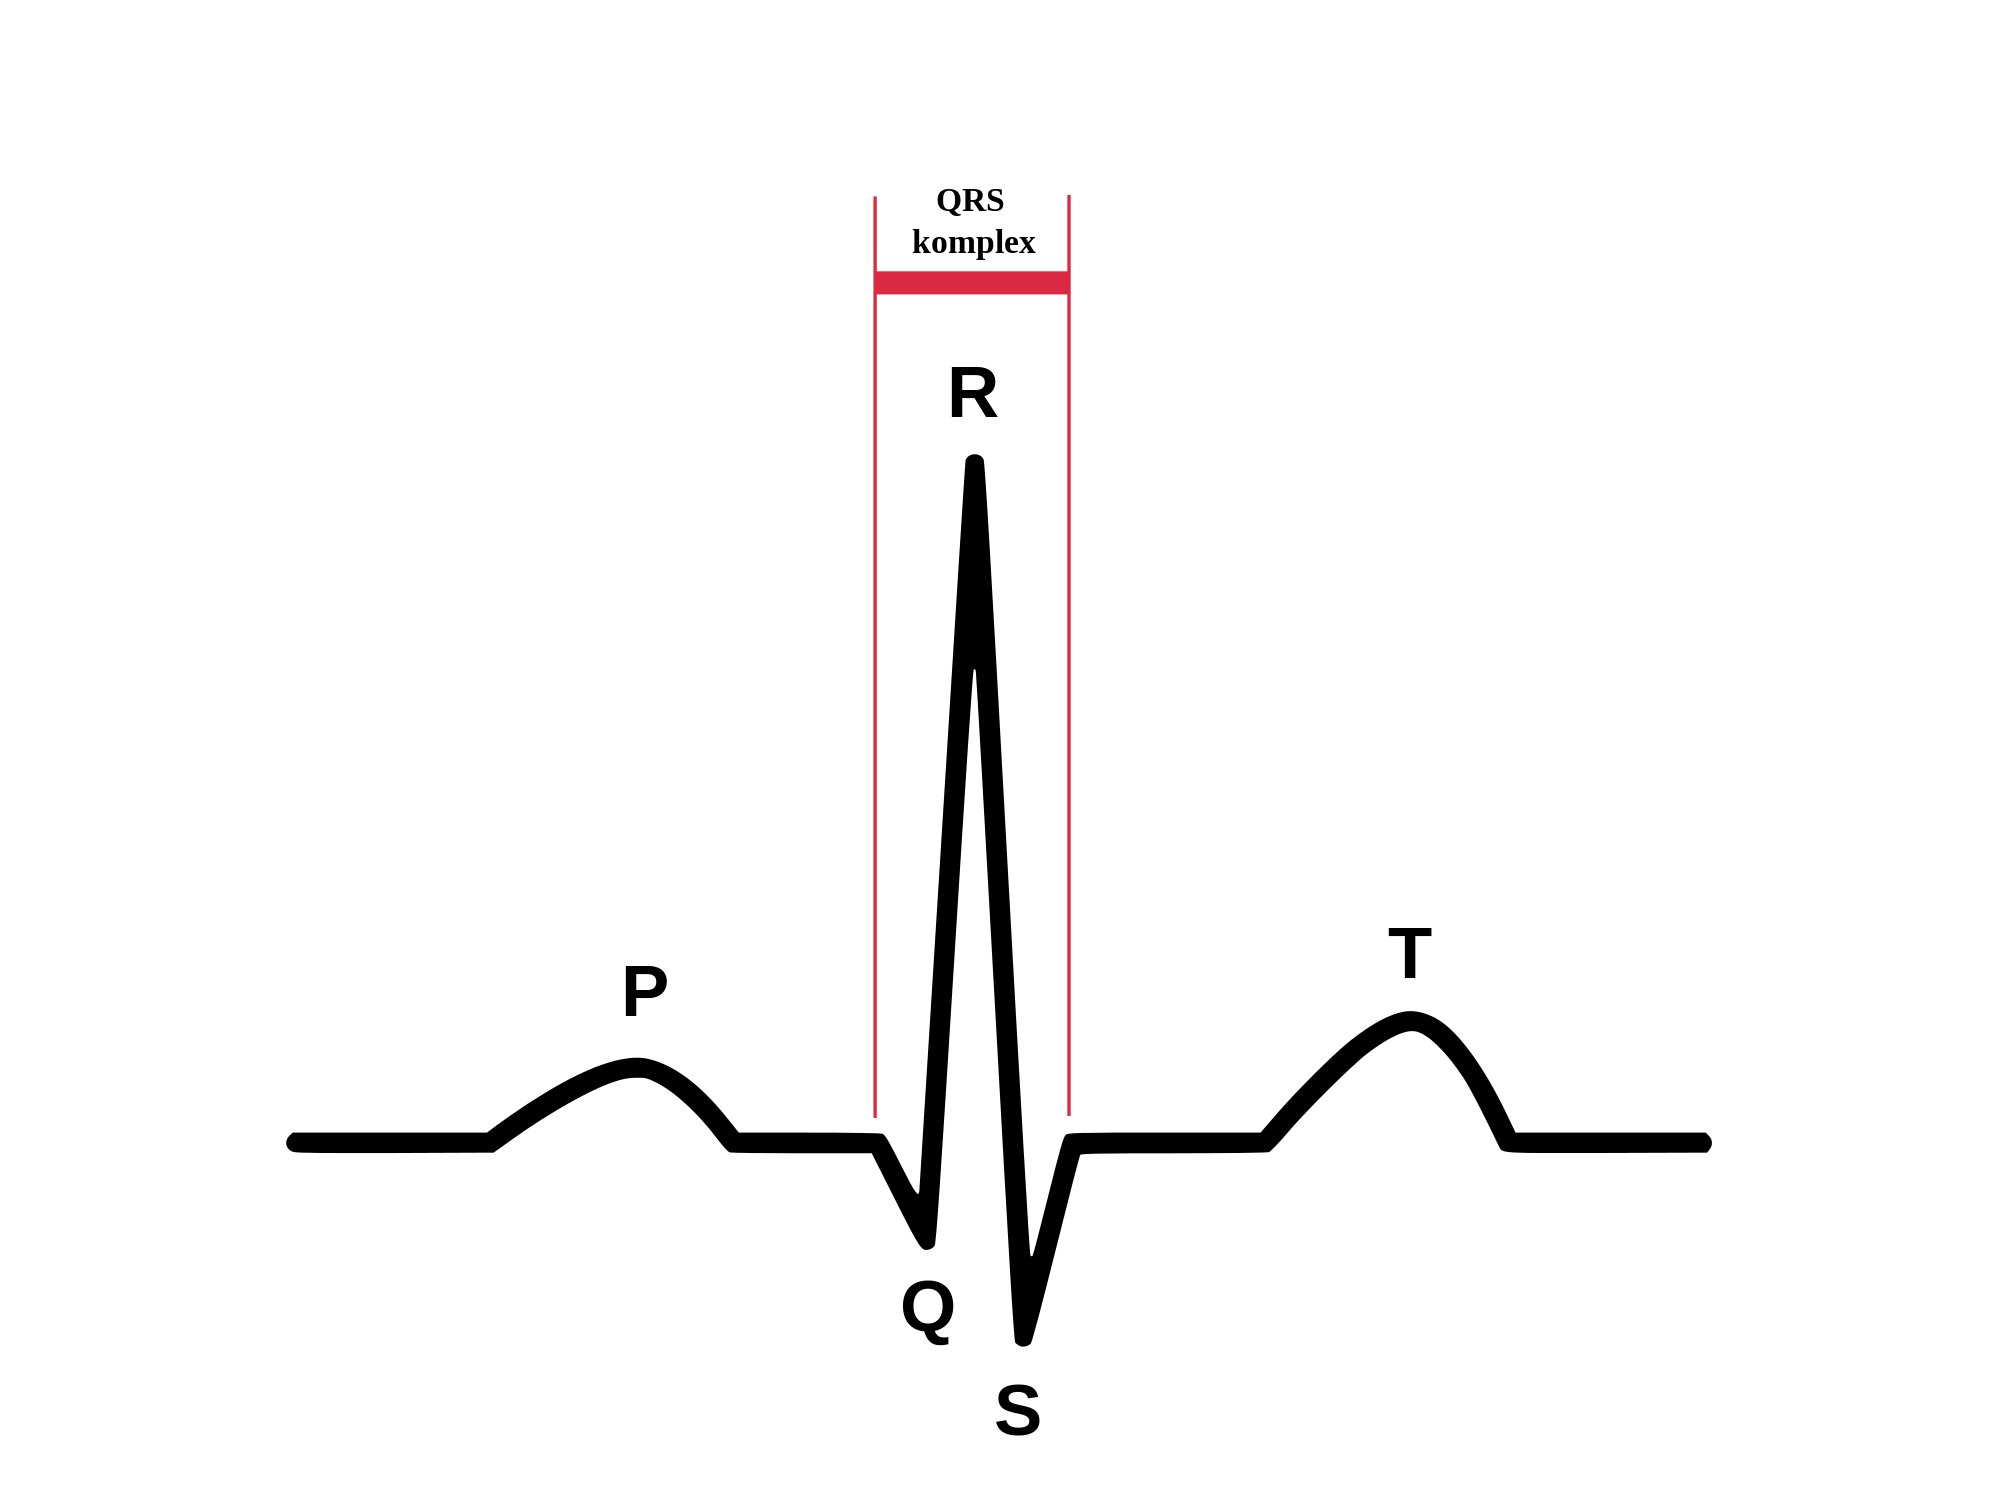
\includegraphics[width=0.9\textwidth]{bilder/b_ecg_pqrst}
     \caption{Illustration of a tetrahedra having 4 vertex points, A, B, C and D}.
     \label{b_ecg_pqrst.png}
\end{figure}

Despite the commonly used ECG, and other methods such as an MRI scan, there are still many questions that yet remains unsolved. According to [HEART BOOK] there is an remarkable knowledge of the heart on the cellular and sub-cellular level, although, the process of connecting the dots for the smale-scale processes that eventually makes a fully functional heart is more difficult. An example of a complex process that researchers have a limited understanding of is defibrillation \cite{article24}. Defibrillation is an electrical shock that is applied to end ventricular fibrillation, which is a state that makes the heart produce uncoordinated electrical waves in the ventricles. As a result of ventricular fibrillation, the heart is unable to contract effectively, which leaves the heart unable to pump blood properly \cite{article24}. 

If the smale-scale processes for the cases such as defibrillation could be described in terms of mathematical models, the task of combining the mathematical models into a full model that describes the complete process, is a viable approach. The mathematical models are later solved on a computer. A mathematical model that is used to reproduce e.g a physical behaviour is referred to as a computer simulation. By simulating a pathological condition in the heart such as fibrillation, can lead to a better understanding of the complex process.  Although, keep in mind that the interaction between the different different smale-scale processes that eventually makes a complete description of the heart is a complex and time consuming process, that opposes a serious computational challenge.

The method of simulating the heart in a structured manner has not yet been tested and documented thoroughly. The new structured method of simulating the heart are of great interest to ongoing research activities at the Cardiac Modeling Department at Simula 

\section{The Mathematical Model}
